% Typography matched to the MSc dissertation PDF (Georgia body, 1.5 line spacing,
% A4 with 25 mm side margins, Georgia Bold headings, italic running header, centred page number).
% Georgia is not redistributable; Gelasio (SIL OFL, metric-compatible with Georgia) is used instead.
% Build with XeLaTeX:  xelatex main.tex  (twice).  Default 11 pt = 29 pages; 10 pt = 25 pages; 14 pt = dissertation size.
\documentclass[a4paper]{article}
\usepackage{fontspec}
\ifdefined\bodysize\else\def\bodysize{11}\fi      % body size (pt); the dissertation itself uses 14
\ifdefined\bodyskip\else\def\bodyskip{16.6}\fi   % baseline-to-baseline (pt), 1.5 line spacing as in the dissertation (21.12 at 14 pt)
\defaultfontfeatures{Ligatures=TeX}
\setmainfont{Gelasio}[Path=./fonts/,Extension=.ttf,UprightFont=*-Regular,BoldFont=*-Bold,ItalicFont=*-Italic,BoldItalicFont=*-BoldItalic]
\newfontfamily\headerfont{LiberationSerif}[Path=./fonts/,Extension=.ttf,UprightFont=*-Regular,BoldFont=*-Bold,ItalicFont=*-Italic,BoldItalicFont=*-BoldItalic]
\setmonofont{LiberationMono}[Path=./fonts/,Extension=.ttf,UprightFont=*-Regular,BoldFont=*-Bold,ItalicFont=*-Italic,BoldItalicFont=*-BoldItalic,Scale=MatchLowercase]
\usepackage{xfp}
\newcommand{\sz}[1]{\fpeval{#1*\bodysize/14}}     % scale a dissertation point size
\renewcommand{\normalsize}{\fontsize{\bodysize}{\bodyskip}\selectfont}
\renewcommand{\small}{\fontsize{\sz{11.7}}{\sz{15.6}}\selectfont}
\renewcommand{\footnotesize}{\fontsize{\sz{10}}{\sz{13}}\selectfont}
\normalsize
\setlength{\parindent}{\fpeval{21.1*\bodysize/14}pt}   % first-line indent as in the dissertation
\setlength{\parskip}{0pt}
\setlength{\emergencystretch}{2em}
\usepackage[a4paper,left=70.8pt,right=70.5pt,top=72pt,bottom=64pt,headheight=14pt,headsep=28pt,footskip=24pt]{geometry}
\usepackage{microtype}
\usepackage{graphicx}
\usepackage{booktabs}
\usepackage{adjustbox}
\usepackage{amsmath}
\usepackage{amssymb}
\usepackage{etoolbox}
\usepackage{caption}
\DeclareCaptionLabelSeparator{emdash}{ --- }
\DeclareCaptionLabelSeparator{endash}{ -- }
\captionsetup{font={it,footnotesize},labelfont={it,footnotesize},justification=centering,singlelinecheck=false,skip=8pt}
\captionsetup[table]{labelsep=emdash,position=below}
\captionsetup[figure]{labelsep=endash,position=below}
\usepackage{fancyhdr}
\pagestyle{fancy}
\fancyhf{}
\fancyhead[R]{\headerfont\itshape\fontsize{\sz{12.3}}{\sz{14}}\selectfont IN939 LPBF Crack Detection}
\fancyfoot[C]{\thepage}
\renewcommand{\headrulewidth}{0.4pt}
\renewcommand{\footrulewidth}{0pt}
\fancypagestyle{plain}{\fancyhf{}\fancyfoot[C]{\thepage}\renewcommand{\headrulewidth}{0pt}}
\usepackage{titlesec}
% top level = dissertation "chapter" heading; second level = "1.1" heading; third = "3.3.1" heading
\titleformat{\section}{\raggedright\hyphenpenalty=10000\exhyphenpenalty=10000 \fontsize{\sz{20.5}}{\sz{25}}\selectfont\bfseries}{\thesection.}{0.65em}{}
\titleformat{\subsection}[hang]{\raggedright\hyphenpenalty=10000\exhyphenpenalty=10000 \fontsize{\sz{20.5}}{\sz{25}}\selectfont\bfseries}{\makebox[2.58em][l]{\thesubsection}}{0pt}{}
\titleformat{\subsubsection}[hang]{\raggedright\hyphenpenalty=10000\exhyphenpenalty=10000 \fontsize{\sz{17}}{\sz{21}}\selectfont\bfseries}{\makebox[3.5em][l]{\thesubsubsection}}{0pt}{}
\titlespacing*{\section}{0pt}{\sz{34}pt}{\sz{22}pt}
\titlespacing*{\subsection}{0pt}{\sz{28}pt}{\sz{18}pt}
\titlespacing*{\subsubsection}{0pt}{\sz{24}pt}{\sz{12}pt}
\usepackage{etoolbox}
\usepackage{chngcntr}
\counterwithin{table}{section}
\counterwithin{figure}{section}
\usepackage[authoryear,round]{natbib}
\setlength{\bibhang}{34pt}
\setlength{\bibsep}{\sz{5}pt}
\usepackage[hidelinks]{hyperref}

\title{\textbf{Explainable Crack-Risk Estimation in IN939 Laser Powder Bed Fusion from Literature-Mined Process Data and Acoustic-Emission Proxy Classification}}
\author{Khushbu Kapade\\[2pt]
\small WMG, University of Warwick, Coventry, United Kingdom}
\date{}

\begin{document}
\maketitle

\section*{Abstract}
Inconel 939 (IN939) is a $\gamma'$-strengthened nickel superalloy that is highly susceptible to solidification, liquation and strain-age cracking during Laser Powder Bed Fusion (LPBF). Crack detection currently relies on slow, expensive or destructive ex-situ methods such as CT scanning and metallography. This paper asks whether in-situ sensor evidence, published process knowledge and explainable machine learning can together give a cheaper indication of crack risk when confirmed ground-truth labels are unavailable. We use a three-stream design. Stream~1 applies a physics-based proxy classification to ten real acoustic-emission (AE) recordings, using a modified $z$-score outlier test and a dual-channel burst-and-collapse search, and treats one thermal recording descriptively. Stream~2 builds a 129-sample literature dataset from ten published IN939 LPBF studies with an LLM-assisted extraction pipeline that retains an evidence quotation for every field. Stream~3 trains a Random Forest classifier on this dataset, validates it with stratified five-fold cross-validation, and interprets it with SHAP. In the literature, 114 of 129 conditions (88.4\%) report cracking. The classifier reaches 92.2\% cross-validated accuracy, but only 0.65 precision and 0.73 recall on the minority no-crack class, against an 88.4\% majority-class baseline. SHAP ranks chemical doping status as the strongest predictor, ahead of layer thickness and well ahead of volumetric energy density (VED). In Stream~1, one recording shows a high-confidence fracture-like signature and two more show medium-confidence signatures. These proxy classifications are not confirmed detections. We report the limits of every stream explicitly and argue that, when labels are scarce, evidence of different status should be reported separately rather than blended.


\medskip\noindent\textbf{Keywords:} IN939; laser powder bed fusion; crack detection; acoustic emission; explainable machine learning; SHAP; large language models; literature mining

\section{Introduction}
\subsection{Background and Industrial Context}
Additive manufacturing (AM) has moved, over roughly two decades, from rapid prototyping into a production method for high-value, geometrically complex metal components in aerospace, energy and defence. Laser Powder Bed Fusion (LPBF) builds components layer by layer from metal powder, fused locally by a laser, enabling internal channels and near-net-shape parts that are impossible to machine conventionally. Nickel-based superalloys are an obvious fit, since they are used precisely in the high-temperature, high-stress applications where the geometric freedom of AM matters most. AM also makes it possible to consolidate several conventionally machined or cast parts into a single printed component, which reduces assembly weight, joints and potential leak paths in turbine hardware.

Inconel 939 (IN939) is one such superalloy: a gamma-prime ($\gamma'$) strengthened, cast nickel superalloy originally developed for turbine components, valued for strength, creep resistance and oxidation resistance up to around 900\,$^\circ$C. These same properties make IN939 one of the harder superalloys to process by LPBF. Its wide solidification range, high $\gamma'$ volume fraction and low-melting eutectic phases at grain boundaries combine to make it highly prone to cracking, a difficulty generally described in the literature as poor ``weldability''. Alloys of this type are often ranked using empirical weldability indices based on aluminium and titanium content, and IN939 consistently falls into the ``difficult to weld/print'' category alongside other high-$\gamma'$ alloys such as Ren\'e~80 and IN738LC. This shared classification means that lessons learned for IN939 crack risk may transfer, at least qualitatively, to a broader family of difficult-to-print nickel superalloys rather than being an isolated case specific to one alloy composition.

For an organisation qualifying IN939 LPBF components, cracking is not cosmetic. It threatens mechanical integrity and creep life, and undetected cracks in a rotating turbine component could have severe safety consequences, potentially propagating under cyclic thermal and mechanical loading in service long after the part has passed initial inspection. Current detection relies overwhelmingly on ex-situ, post-build methods: microscopy, X-ray CT scanning and destructive mechanical testing. All are effective but slow, expensive and, in two of the three cases, destructive. CT scanning, while non-destructive, requires specialist equipment and can take hours per part, which scales poorly to production or to rapid parameter-development work where dozens of trial builds may be needed to converge on a workable process window.

A further barrier compounds this. AM parts, built layer by layer without the long-established property database of wrought or cast stock, typically require substantially more qualification evidence before acceptance into safety-critical applications, and every additional inspection step adds cost and lead time. IN939 sits at a particularly awkward point: its high-temperature properties are exactly what make it attractive for AM, yet its crack-proneness is exactly what makes it hardest to qualify with confidence. This paper does not try to solve that broader qualification challenge. Instead, it looks at one concrete piece of it: whether cheaper, faster evidence of crack risk, even evidence that falls short of full qualification-grade certainty, can usefully inform where expensive, slower inspection should be targeted, so that limited CT and metallography capacity is spent on the builds most likely to need it.

\subsection{The Case for In-Process Monitoring}
An alternative, increasingly explored across the AM research community, is in-situ monitoring: instrumenting the printer with sensors (thermal cameras, acoustic-emission (AE) transducers, melt-pool cameras) that record continuously during the build, in the hope that the resulting signals carry a detectable signature of defect formation as it happens rather than after the fact. If a crack-forming event produces a distinctive acoustic or thermal signature, a monitoring system could flag it during the build, allowing intervention or targeted post-build inspection rather than blind reliance on process parameters alone. Such monitoring is also attractive because the underlying sensors are comparatively inexpensive relative to CT equipment and can, in principle, be retrofitted to an existing printer without disrupting the build process. CT scanning can only happen once the build is done and the part has come off the machine; in-situ monitoring raises the possibility of spotting a problem while it is still developing, when one can still pause, adjust or abort.

This work sits between research threads that, for IN939, have mostly been kept apart. One is process-parameter studies, working out which combinations of laser power, scan speed, hatch spacing and layer thickness (often summarised as Volumetric Energy Density, VED) tend to cause cracking. The other is sensor-monitoring studies, which try to catch defects directly from AE or thermal signals as the build happens. A third thread uses machine learning not only to predict outcomes but to explain which factors drive predictions, via techniques such as SHAP. This motivates the emphasis on interpretability here, since a black-box prediction of ``high risk'' is of limited practical use to a process engineer without some indication of which parameter to change first.

\subsection{Problem Statement}
The practical starting point was a specific real dataset from the project's laboratory contact: ten raw AE recordings and one thermal-camera recording from real IN939 LPBF-related test activity, together with the published IN939 powder-bed-fusion literature. Critically, the real sensor recordings came with no confirmed record of which, if any, corresponded to a specimen that actually cracked. This was never logged at the time, and the laboratory contact does not have access to it. This absence of ground truth is the central practical obstacle the work had to be designed around, and we document the reasoning and supervisor-approved decisions used to do so honestly rather than by fabricating labels.

Put simply: there are real multi-sensor recordings with no confirmed labels, and a body of published research reporting labelled outcomes across various process conditions. Can physics-informed signal analysis, combined with machine learning trained on that literature, turn those two things into a crack-risk estimate that is defensible, explainable and does not overstate what it knows, given that none of the actual specimens has confirmed ground truth? With data this scarce, being honest about the limits of the estimate matters as much as getting the signal processing or the model right. The problem is also deliberately narrower and more tractable than ``build a production-ready crack detector'': the goal is to establish whether the available evidence, honestly combined, can support a defensible risk estimate at all, leaving formal validation to future work.

\subsection{Aim and Objectives}
The aim is to design, build and critically evaluate a multi-stream approach to assessing crack risk in IN939 LPBF components, one that brings together real sensor-signal analysis, literature-derived process knowledge and explainable machine learning, while staying honest about the fact that confirmed ground truth is not available. The objectives are:
\begin{itemize}
  \item to review and synthesise the published literature on cracking mechanisms, process-parameter effects and mitigation strategies (including compositional doping) in IN939 processed by LPBF;
  \item to design and implement a physics-based method for inferring likely fracture events directly from raw acoustic and thermal sensor recordings in the absence of recorded ground truth, and apply it to all available real recordings;
  \item to build a structured, quality-checked dataset of process parameters and crack outcomes from published IN939 LPBF studies using an LLM-assisted literature-mining pipeline, sufficient to support supervised machine learning;
  \item to train and rigorously validate a machine learning classifier on this dataset, using cross-validation appropriate to its size and class imbalance, and apply SHAP to interpret its predictions;
  \item to apply the trained model to the real specimens available, using the best estimate of their process parameters, and compare this against the sensor-signal proxy classification; and
  \item to document transparently the limitations of every method used, distinguishing statistically validated findings from illustrative or exploratory ones.
\end{itemize}
\subsection{Research Questions}
\begin{itemize}
  \item \textbf{RQ1:} What can be inferred about the likelihood of a fracture event directly from the raw shape of acoustic and thermal sensor signals, when no confirmed outcome label exists?
  \item \textbf{RQ2:} Which process parameters, and to what extent, predict cracking in IN939 LPBF according to published evidence, and can a machine learning model trained on that evidence produce accurate, explainable predictions?
  \item \textbf{RQ3:} How should proxy, literature-derived and directly measured evidence be combined and reported when confirmed ground truth is unavailable, in a way that remains scientifically honest about its limitations?
\end{itemize}
The contributions are a physics-based proxy classification of raw AE recordings that works without outcome labels and flags every output as unconfirmed; a structured 129-sample dataset mined by an LLM pipeline that records an evidence quotation per field; a cross-validated Random Forest with SHAP analysis showing that doping status outweighs VED and the individual process parameters in the pooled literature; and an explicit scheme for reporting validated findings, proxy inferences and estimate-based illustrations separately. We do not claim a novel signal-processing algorithm or model architecture, and we do not claim a deployable crack detector.

\subsection{Structure of the Paper}
Section~2 reviews the literature on IN939 LPBF processing, cracking mechanisms, mitigation strategies, in-situ monitoring and machine learning for defect prediction, and identifies the specific gap addressed. Section~3 lays out the methodology across all three streams, including the proxy-labelling approach and the two methodological decisions approved by the supervisor. Section~4 presents the results, Section~5 discusses them together with their limitations, and Section~6 concludes and sets out future work.

\section{Literature Review}
\subsection{IN939 and the Laser Powder Bed Fusion Process}
LPBF builds metal parts by repeatedly spreading a thin layer of powder (typically 20--60\,$\mu$m) and selectively melting it with a laser following a sliced 3D model path. The key process parameters (laser power, scan speed, hatch spacing and layer thickness) are frequently combined into the Volumetric Energy Density (VED), in J/mm$^3$:
\begin{equation}
  \mathrm{VED} = \frac{P}{v\,h\,t},
\end{equation}
where $P$ is laser power (W), $v$ is scan speed (mm/s), $h$ is hatch spacing (mm) and $t$ is layer thickness (mm). VED is widely used across the LPBF literature as a first-order summary of the thermal energy delivered per unit volume, and is frequently plotted against measured density or defect rate to identify a usable process window, though, as shown below, VED alone does not fully capture crack risk. It is popular because it condenses four independently adjustable machine settings into a single number that can be swept across a design-of-experiments grid, but this convenience comes at the cost of discarding information about which of the four parameters is responsible for a given outcome. The feature set used here (Section~3.5) therefore retains the individual parameters alongside VED.

IN939 is a cast, precipitation-hardened superalloy strengthened mainly by $\gamma'$ (Ni$_3$(Al,Ti)), along with chromium, cobalt, tungsten, tantalum, aluminium and titanium. Developed for investment-cast turbine components up to roughly 900\,$^\circ$C, its high $\gamma'$ content and moderate carbides give strong creep and oxidation resistance. These same features make it difficult to process by any fusion-based method: high $\gamma'$-forming content promotes strain-age cracking during post-weld heat treatment, while a wide solidification range and grain-boundary eutectic segregation promote solidification and liquation cracking during the rapid thermal cycling of LPBF \citep{marchese2020,dogu2024}. The repeated heating and cooling inherent to LPBF, often exceeding $10^3$--$10^6$\,$^\circ$C/s locally, is itself a departure from the slower, more controlled thermal histories the alloy was originally designed around. Cast IN939 solidifies slowly and relatively uniformly within a mould, allowing time for stress to relax and for segregated elements to partially redistribute; LPBF instead builds the same alloy through thousands of rapid, highly localised melt-and-resolidify events, so the metallurgical behaviour that has made IN939 a reliable casting alloy for decades does not transfer straightforwardly to a fundamentally different thermal process.

\subsection{Cracking Mechanisms in LPBF-Fabricated IN939}
The literature converges on three mechanisms that frequently co-occur. Solidification cracking occurs within the still-solidifying ``mushy zone'', where tensile strain from shrinkage and thermal contraction exceeds the strength of the partially solid network while a liquid film persists along boundaries \citep{ozer2024}. Liquation cracking occurs in previously solidified material reheated by subsequent layers, causing incipient melting of low-melting precipitates or eutectic regions at grain boundaries, which residual stress then tears open. Strain-age cracking occurs during post-build heat treatment, when reheating a $\gamma'$-strengthened alloy drives rapid $\gamma'$ precipitation that stiffens the matrix and relieves residual stress; if the resulting strain exceeds the reduced ductility of the freshly hardened matrix, cracking results \citep{ozer2024}. Because each mechanism is tied to a different stage of the thermal history (during solidification, during subsequent layer deposition, or during post-build heat treatment), a build that appears sound immediately after printing can still develop new cracks later in its processing route. A single CT scan performed immediately after printing, before heat treatment, may therefore miss strain-age cracks that only develop during the subsequent thermal cycle, which makes post-heat-treatment inspection arguably the more decisive checkpoint for components destined for service.

\citet{ozer2024} compared as-fabricated IN939 against two post-build aging treatments, finding that both increased microhardness (339.8\,$\pm$\,3.4\,HV as fabricated, 440.2\,$\pm$\,5.6\,HV after a first treatment, 508.1\,$\pm$\,4.8\,HV after a second) via $\gamma'$ coarsening and carbide transformation, but at the cost of introducing new liquation and strain-age cracking. This shows that crack risk is not simply a function of as-built parameters: post-processing heat treatment can itself introduce new cracking. It is why the literature dataset used here records crack occurrence per sample rather than assuming one label per build, and why any future extension would need to record the heat-treatment state of each reported sample explicitly.

All ten source papers mined for this work report the same family of crack types, a consistency across independent groups that supports treating IN939's crack-proneness as a genuine material property rather than a laboratory-specific artefact. Solidification cracking is reported in all ten sources; liquation cracking in three \citep{ozer2024,marchese2020,hu2024}, in the case of \citet{hu2024} via ductility-dip cracking; and strain-age cracking in two \citep{ozer2024,hu2024}. Residual stress from thermal cycling is cited in nine of ten, and segregation of titanium, tantalum, niobium, zirconium and carbon to grain boundaries in eight of ten. This near-unanimous agreement across studies using different printers, powders and parameter ranges suggests that the dominant cracking mechanisms are governed more by the alloy's intrinsic solidification chemistry than by any single facility's equipment or practice. Notably, all ten sources characterise cracking exclusively via ex-situ, post-build methods: optical or SEM microscopy in all ten, EBSD in seven, EDS/EDX in eight, XRD in six and CT scanning in only two \citep{zhang2023,bae2025}. None reports using acoustic emission, thermal imaging or any in-situ sensing at all, confirming the research gap addressed here: in-situ monitoring and process or compositional characterisation have been pursued separately for this alloy, and no source in this review attempts to relate a real-time sensor signal back to a subsequently confirmed metallurgical crack finding for IN939 specifically. This is not unique to IN939 and reflects a broader pattern across nickel-superalloy LPBF research: compositional and process studies tend to be carried out by metallurgy-focused groups, while in-situ sensing studies tend to come from process-monitoring or manufacturing-engineering groups, and there is comparatively little cross-disciplinary work connecting the two for any given alloy.

\subsection{Effect of Process Parameters and Volumetric Energy Density}
\citet{marchese2020} systematically varied scan speed and hatch distance and found that porosity and cracking cannot be minimised independently: settings that minimise one do not necessarily minimise the other, which is why the dataset used here records them as separate outcomes. \citet{dogu2024} extended this to laser power, scan speed and hatch distance, confirming a narrow but real defect-minimising process window. \citet{li2024} found that alloying-element segregation and residual stress, rather than energy density alone, are the more fundamental drivers, and showed that substrate preheating reduces cracking even at otherwise crack-prone energy densities. \citet{rodriguezbarber2023} showed that switching from continuous-wave to pulsed-wave laser emission changes microstructure and mechanical behaviour. \citet{hu2024} found that laser remelting, rescanning a layer before the next is applied, reduces both cracking and porosity via residual-stress relief and refined dendritic structure.

Specific parameter values illustrate how narrow the window is. \citet{marchese2020} report 1800\,mm/s scan speed with 0.03\,mm hatch distance minimising crack density, while 1000\,mm/s at the same hatch distance instead minimised porosity: two different optima from the same shared parameter, so any single ``optimal'' recipe necessarily trades one defect type against the other unless a third lever, such as doping, is introduced. \citet{rodriguezbarber2023} bracket their usable VED range between 43 and 60\,J/mm$^3$. \citet{li2024} report a range of 37.5--58.3\,J/mm$^3$, with 180\,$^\circ$C preheating raising UTS from 1082.5 to 1118.1\,MPa, yield strength from 857.0 to 883.6\,MPa, and elongation from 13.76\% to 15.26\%. \citet{chen2026}, studying TiC-modified IN939, report an optimum at 240\,W, 1400\,mm/s, 70\,$\mu$m spacing and 30\,$\mu$m layer thickness (VED $\approx 81.63$\,J/mm$^3$), within the same broad 40--90\,J/mm$^3$ region on which other studies converge despite different platforms, powders and, in several cases, different laser types. That this broad range recurs across studies using different equipment lends it some credibility as a genuine material characteristic of IN939 rather than an artefact of any one facility's calibration, though the persistent disagreement about the precise optimum within that range is itself evidence that VED is an incomplete descriptor of the underlying physics.

Together, this body of work shows that VED is necessary but not sufficient for predicting crack risk. Substrate preheating, laser emission mode and remelting each shift outcomes independently at a given VED, so two studies with broadly overlapping VED ranges can still report meaningfully different cracking behaviour depending on these secondary choices. This is why the model of Section~3.5 includes the individual process parameters alongside VED, rather than assuming VED alone summarises the process, so that it can pick up interactions a single composite metric would hide. It also has a practical implication: a reported ``safe'' VED range from one paper should not be transferred uncritically to a different printer, powder batch or preheating regime without accounting for these secondary factors, since outcomes can diverge meaningfully even at nominally similar VED values.

\subsection{Compositional Modification and Doping Strategies}
A second research thread modifies the alloy composition directly, introducing a secondary phase or grain-refining element to suppress cracking at its metallurgical root rather than tuning around it with laser settings. This is conceptually distinct from the process-parameter thread: rather than searching for a narrow safe window within the alloy's existing chemistry, doping strategies attempt to widen that window, or eliminate the crack-driving mechanism altogether, by changing the solidifying liquid's own behaviour.

\citet{zhang2023} found that silicon addition substantially reduces solidification cracking, a result running contrary to some prior expectations, attributed to Si's effect on interdendritic liquid-film characteristics. \citet{chen2026} added 1\,wt\% TiC particles, which act as nucleation sites, refining grain structure and suppressing cracking while improving densification. \citet{bae2025} reported an even stronger effect with TiB$_2$ addition, eliminating cracking entirely while improving mechanical properties at room and elevated temperature, among the strongest single mitigation results reviewed. \citet{ding2026} combined silicon and yttria (Y$_2$O$_3$), reporting fully crack-free builds, an improved strength--ductility balance, randomised grain orientation and better oxidation resistance at 1200\,$^\circ$C. This suggests dual doping may address cracking and oxidation performance simultaneously, which would be valuable for turbine applications, since a component that resists cracking during manufacture but oxidises prematurely in service would still be an incomplete solution.

These improvements are substantial. \citet{zhang2023} report nanoindentation hardness rising from $\sim$5.9\,GPa to $\sim$6.4\,GPa with 3\% silicon. \citet{chen2026} report tensile strength rising from 560 to 699\,MPa (+24.82\%) with TiC, alongside a 25.51\% yield-strength gain and increased elongation. \citet{bae2025} report yield strength rising from $\sim$600 to 1256\,MPa and UTS from $\sim$800 to 1578\,MPa with TiB$_2$, comparable to wrought superalloys, a striking result given that undoped LPBF IN939 is generally reported as brittle and crack-prone. The dual-doped material of \citet{ding2026} shows the most striking figure reviewed: elongation rising from $0.21\pm0.03\%$ (near-brittle) to $10.0\pm0.2\%$ with silicon alone and $12.1\pm0.4\%$ combined, with UTS rising from 968.33 to 1171.26\,MPa. An elongation improvement of this scale is a direct signature of crack suppression, consistent with the grain-boundary mechanisms of Section~2.2 being substantially suppressed rather than merely reduced in frequency. Taken together, these four doping studies suggest a general principle rather than four isolated results: introducing a secondary phase or grain refiner that disrupts the continuous liquid film along solidifying grain boundaries appears to be an effective lever against IN939 cracking regardless of the specific dopant chosen, though each dopant brings its own trade-offs in cost, processability and effect on other properties that a production decision would need to weigh.

Table~\ref{tab:sources} summarises cracking rates against doping status across all ten sources. The three non-doped process-parameter studies of \citet{dogu2024}, \citet{marchese2020} and \citet{li2024} report cracking in every sample (27/27, 48/48 and 3/3). Of the four sources that include doped samples, three report materially lower crack proportions (\citealt{zhang2023}, 2/3; \citealt{ding2026}, 1/3; \citealt{bae2025}, 4/12), while in \citet{chen2026} both samples cracked (2/2), only one of them doped.

\begin{table}[t]
\centering
\small
\begin{adjustbox}{max width=\textwidth,center}
\begin{tabular}{lccc}
\toprule
Source (topic) & Samples & Reporting cracking & Doped samples \\
\midrule
Doğu et al.\ (2024), process parameters & 27 & 27 (100\%) & 0 \\
Marchese et al.\ (2020), process parameters & 48 & 48 (100\%) & 0 \\
Li et al.\ (2024/2025), preheating & 3 & 3 (100\%) & 0 \\
Rodr\'iguez-Barber et al.\ (2023), pulsed wave & 27 & 23 (85\%) & 0 \\
Ozer et al.\ (2024), aging treatment & 3 & 3 (100\%) & 0 \\
Hu et al.\ (2024), remelting & 1 & 1 (100\%) & 0 \\
Zhang et al.\ (2023), Si addition & 3 & 2 (67\%) & 2 \\
Chen et al.\ (2026), TiC addition & 2 & 2 (100\%) & 1 \\
Ding et al.\ (2026), Si + Y$_2$O$_3$ & 3 & 1 (33\%) & 2 \\
Bae et al.\ (2025), TiB$_2$ addition & 12 & 4 (33\%) & 8 \\
\midrule
Total & 129 & 114 (88.4\%) & 13 \\
\bottomrule
\end{tabular}
\end{adjustbox}
\caption{Reported crack outcomes by source paper.}
\label{tab:sources}
\end{table}

\begin{figure}[t]
\centering
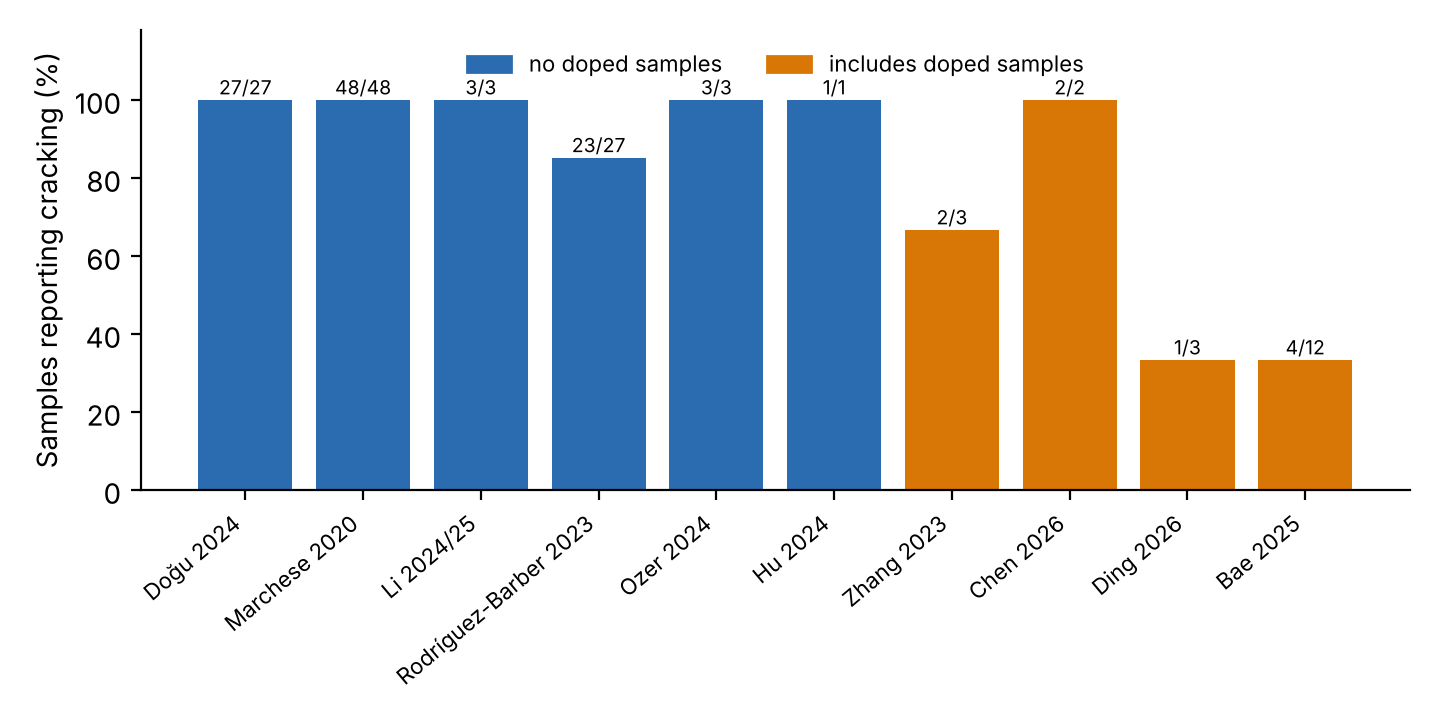
\includegraphics[width=0.85\textwidth]{figs/fig_crack_rate_by_paper.png}
\caption{Percentage of samples reporting cracking by source paper, computed from the Stream~2 dataset (matches Table~\ref{tab:sources}). Labels give cracked/total counts.}
\label{fig:crackrate}
\end{figure}

This pattern directly informs Stream~3: doping status is included as a categorical feature and, as Section~4 reports, emerges from SHAP analysis as the most influential feature, ahead of VED, consistent with the qualitative pattern already visible across these papers before any model is trained.

\subsection{In-Situ Process Monitoring in Metal Additive Manufacturing}
A separate research thread asks whether defects can be detected directly from sensor signals recorded during the build, rather than inferred from process settings or confirmed after the fact. \citet{grasso2017}, in a widely cited review, catalogue the in-situ sensing modalities used in metal powder bed fusion (optical and thermal melt-pool imaging, acoustic and vibration sensing) along with the signal-processing methods used to turn raw streams into defect indicators. AE sensing detects transient elastic waves released by a sudden, localised release of strain energy (crack initiation, plastic deformation, phase transformation), a well-established non-destructive technique applied more recently to AM. \citet{wasmer2019} demonstrated an in-situ AM quality-monitoring system using AE combined with reinforcement learning, distinguishing build-quality outcomes without destructive post-build inspection. This illustrates that AE carries genuinely useful information about build quality even without a full physical model of the melt pool, and is an important precedent: meaningful process information can be extracted from AE signals using comparatively lightweight signal-processing and learning methods, without the high-fidelity physics simulation that would be needed to model melt-pool behaviour from first principles.

The physical principle underlying AE-based detection is that a genuine fracture produces a large, often multi-sensor-detectable amplitude burst, distinct from ordinary elastic or plastic deformation, typically followed by a collapse in subsequent activity. This is exactly what Stream~1 (Section~3.3) applies directly to the real AE recordings. This work does not advance AE signal-processing theory; it applies established physical reasoning to a situation the literature does not directly address: recordings with no confirmed outcome label at all, rather than the more common situation of training a classifier from labelled examples. This distinction is not a minor technicality. The vast majority of published AE-based defect-detection work assumes labelled training data is available, and comparatively little addresses how to make responsible use of AE data when it is not. Our position is that this gap should not simply be left unaddressed until labelled data becomes available: engineering organisations frequently hold exactly this kind of unlabelled sensor archive already, and a transparent, physically grounded method for extracting partial value from it, clearly flagged as a proxy rather than a validated detector, is preferable to leaving that data unused indefinitely while waiting for a labelling exercise that may never happen.

\subsection{Machine Learning and Explainable AI for Defect Prediction}
Supervised machine learning applied to AM process--outcome prediction has grown rapidly, since mapping dozens of interacting process variables to a defect outcome is exactly the kind of high-dimensional, non-linear relationship that learning approximates well given sufficient labelled examples. Random Forest classifiers \citep{breiman2001} are a common choice for tabular, moderate-sample-size problems, combining strong predictive performance with interpretability via feature importance, which is relevant to a safety-adjacent application where users need to know why a prediction was made, not simply what it is.

SHAP \citep{lundberg2017} has become a widely adopted explanation framework because it attributes each prediction to an additive contribution from each feature, grounded in cooperative game theory, and can be aggregated to summarise overall feature importance in a way that is more theoretically grounded than simpler measures such as raw Gini importance. Stream~3 (Section~3.5) applies SHAP to answer a question directly motivated by Sections~2.3 and~2.4: given that both process parameters and compositional doping are independently reported to affect crack outcomes, which category matters more according to a model trained across the literature as a whole, rather than within any single paper's own narrower parameter range? This could in principle be answered qualitatively by reading the ten papers side by side, but a model trained jointly across all 129 samples, combined with SHAP's game-theoretic attribution, provides a quantitative answer: a ranked, numerically comparable measure of relative influence that a purely narrative synthesis cannot offer on its own.

\subsection{Research Gap and Positioning of This Paper}
The review reveals two absences. First, none of the process-parameter or doping studies incorporates in-situ sensor monitoring (they establish outcomes exclusively via post-build inspection), and none combines that literature with a trained model applied back to sensor-monitored specimens. Second, the in-situ monitoring literature, while establishing the physical basis for AE-based detection, is not designed for a situation where real specimens carry no confirmed ground-truth label at all: existing approaches, including that of \citet{wasmer2019}, are trained and evaluated against known labels, which are unavailable here.

The contribution is therefore not a novel signal-processing algorithm or model architecture, each of which would require resources (confirmed ground-truth labelling, new print trials) genuinely unavailable within this project's constraints. Rather, it is a methodologically transparent demonstration of how existing process-parameter and doping literature, combined via an explainable model and cross-referenced against a physics-based reading of real but unlabelled sensor data, can together produce an actionable, explained crack-risk estimate, explicit at every step about which parts are statistically validated and which are illustrative.

\section{Methodology}
\subsection{Overall Research Design}
The work adopts a three-stream design (Table~\ref{tab:streams}), since no single available dataset was independently sufficient to answer the research questions. The real sensor recordings (ten AE recordings, one thermal recording) are genuine but carry no confirmed outcome label and are far too few to train or validate a supervised model. The literature provides 129 labelled samples, enough for training, but describes other laboratories' builds. The design uses each source for the task it suits: real sensor data for direct physics-based signal reading (Stream~1); literature data for model training (Stream~2, feeding Stream~3); and the trained model applied back to real specimens as a second, independent estimate alongside Stream~1 (Section~3.5.3). This division of labour was chosen deliberately over the alternative of forcing one dataset to serve all three roles, which would have required either fabricating labels for the real data or ignoring it entirely. An early alternative design considered training a model directly on the ten real recordings using Stream~1's proxy classifications as labels. This was rejected specifically because it would have circularly validated the proxy method against itself rather than providing any independent check, and because ten examples are simply too few to train a supervised model with any confidence regardless of label quality.

\begin{table}[t]
\centering
\small
\begin{adjustbox}{max width=\textwidth,center}
\begin{tabular}{p{1.3cm}p{3.4cm}p{4.4cm}p{3.4cm}}
\toprule
Stream & Input data & Core method & Output \\
\midrule
1 & 10 real AE recordings; 1 thermal recording & Modified $z$-score outlier test; dual-channel burst detection & Proxy fracture classification per recording, with confidence \\
2 & 10 published IN939 LPBF papers & LLM-assisted structured extraction, cleaning and QC & 129-sample labelled literature dataset \\
3 & Stream~2 dataset; estimated specimen parameters & Random Forest, stratified 5-fold CV, SHAP & CV performance, feature importance, specimen prediction \\
\bottomrule
\end{tabular}
\end{adjustbox}
\caption{Summary of the three-stream research design: inputs, methods and outputs.}
\label{tab:streams}
\end{table}

\subsection{Data Sources}
Two categories of real data were provided by the project's laboratory contact, from an operational IN939 LPBF printer and test rigs. The first is ten AE recordings: eight AEwin parameter-versus-time plot exports from tensile ``dogbone'' tests, one plot export from an additional rig (``Brompton''), and one full raw AE hit-list export containing 11,771 individually timestamped hits with channel, rise time, hit count, energy and amplitude, at far higher resolution than the summary exports. The second is a single thermal-camera recording (PIX Connect format, about 8.4\,GB) of a print-cooling sequence for density-cube specimens, 35\,min 44\,s long across 57,898 frames. This file's integrity was independently verified before analysis. Its RIFF/AVI header initially appeared inconsistent with its actual size, which we traced to a well-documented 32-bit size-field limitation affecting any AVI file above 4\,GB regardless of corruption. More conclusively, the final frames were decoded directly with ffmpeg, seeking five seconds before the end and decoding the last three frames with zero errors; a corrupted file would fail this test. The recording was therefore treated as complete for analysis rather than discarded on the basis of a misleading header field.

The raw AE hit-list follows the standard AEwin format: each hit is logged as eleven whitespace-separated fields (identifier, date, sub-millisecond timestamp, internal parameters, channel, rise time, hit count, energy, duration, peak amplitude), giving a complete timestamped record for that one recording. This resolution enabled the direct fracture-signature search of Section~3.3.2, unlike the remaining recordings, which have only a pre-aggregated summary trace and are limited to the coarser group-comparison approach. Crucially, none of these recordings came with a recorded outcome label, since inspection outcomes for these sessions were not logged at the time of testing. This absence of ground truth is the single most consequential fact shaping the methodology, addressed in Section~3.6, and is why Stream~1's outputs are described throughout as proxy classifications rather than detections.

The literature dataset (Stream~2) draws on ten peer-reviewed sources identified through targeted search for IN939-specific LPBF studies reporting process parameters and crack or densification outcomes \citep{marchese2020,zhang2023,rodriguezbarber2023,hu2024,ozer2024,dogu2024,li2024,bae2025,chen2026,ding2026}. Once mined and cleaned (Section~3.4), these yielded 129 usable samples spanning a range of printer platforms, powder suppliers and reporting laboratories, which is itself a strength relative to relying on any single facility's data alone. Combining data across ten independent research groups helps average out facility-specific idiosyncrasies (a particular powder batch, calibration quirk or reporting convention) that could otherwise bias a model trained on a single source's data, though it does introduce some heterogeneity in how each source measured and reported its results, addressed through the quality-control steps of Section~3.4.2.

\subsection{Stream 1 --- Sensor Signal Proxy Classification}
\subsubsection{Rationale}
Given the absence of a confirmed label, two options existed: leave this real evidence unused, or infer a defensible estimate directly from each recording's physical characteristics. We adopt the second, since a genuine fracture has a well-established, physically distinctive acoustic signature (Section~2.5), meaning a considered signal reading can produce meaningful information provided it is clearly reported as an inferred proxy rather than confirmed fact. This proxy/ground-truth distinction is treated as a first-class methodological consideration throughout and, as detailed in Section~3.6, was explicitly reviewed and approved by the supervisor before any results were finalised.

\subsubsection{Method}
Two techniques were applied depending on data resolution. For the eight summary-trace exports and the Brompton recording, each peak reading was compared against comparable recordings using a modified $z$-score, robust to outlier distortion since it uses the median and median absolute deviation (MAD) rather than mean and standard deviation:
\begin{equation}
  M = 0.6745\,\frac{x-\mathrm{median}}{\mathrm{MAD}}.
\end{equation}
Following the convention of \citet{iglewicz1993}, a score above 3.5 was treated as a significant outlier warranting ``Proxy-Yes''; between 1.5 and 3.5 as ``Watch'' (inconclusive); near-zero as ``No significant AE activity''; and all others as ``Inconclusive/baseline activity''.

For the one recording with full raw hit-list resolution, a direct fracture-signature search was performed instead: hits were parsed, the session's maximum amplitude identified, and all near-maximum hits examined for near-simultaneous occurrence on both sensor channels, the signature Section~2.5 identifies as characteristic of a genuine fracture and distinct from single-channel noise. Where this dual-channel burst was found together with a subsequent drop in hit rate, the recording was classified high-confidence ``Proxy-Yes''. This second, higher-resolution method was preferred over the $z$-score approach wherever available, since it examines the underlying physical signature directly rather than relying on a purely statistical comparison against other recordings. The thermal recording was explicitly classified ``not assessable via this method'' since it has no acoustic channel; its temperature and cooling-rate characteristics are instead reported descriptively in Section~4 as supporting context rather than as a proxy classification in its own right.

\subsubsection{Output}
Stream~1's output is an eleven-row table (ten AE recordings and the thermal recording) recording, for each: source, rig or specimen type, quantitative basis ($z$-score or burst timing and amplitude), the resulting classification, confidence level, and an explicit ``ground truth confirmed: No'' flag on every row, so that no reader mistakes a proxy for a confirmed result.

\subsection{Stream 2 --- LLM-Assisted Literature Mining}
\subsubsection{Pipeline Design}
Building a dataset large enough for supervised learning meant extracting comparable data (process parameters, crack outcomes, doping status) from ten source papers, each presenting the information differently, in different units, tables and levels of detail. Manual transcription is slow and error-prone at that scale, so an LLM-assisted extraction pipeline was used, built on LangChain driving a general-purpose LLM, to pull out per sample: process parameters, density or porosity, crack occurrence, doping status and dopant, crack type and location, testing methods, and, critically, a supporting evidence quotation from the source text justifying each extracted field. This requirement allows every data point to be spot-checked against its source rather than trusted opaquely, which was essential given that no independent human transcription was performed as a cross-check.

\subsubsection{Quality Control}
Extracted data passed through a consistency check flagging implausible parameter combinations, and a filter removing rows not representing an individually reported sample. This caught a specific extraction error during development, in which background literature ranges quoted by one heat-treatment paper were incorrectly attributed to its own experimental samples; this was fixed via a refined prompt and an explicit code-level filter that cross-checked each extracted sample against the paper's own results tables. VED was then calculated for every sample using Eq.~(1), cross-checked against directly reported values where available, with any large discrepancy flagged for manual review.

\subsubsection{Final Dataset}
The clean dataset comprises 129 samples from ten papers, recording process parameters, VED, density, porosity, crack occurrence and doping status. It is substantially imbalanced: 114 samples (88.4\%) report cracking against 15 (11.6\%) that do not. This is treated throughout as a genuine finding about IN939's process sensitivity rather than a data-collection shortfall; a targeted search for additional no-crack literature did not surface further usable sources, suggesting that crack-free IN939 LPBF conditions remain genuinely rare in the published record rather than simply under-reported.

\subsection{Stream 3 --- Machine Learning Model and Explainability}
\subsubsection{Feature Selection and Model Choice}
A Random Forest classifier \citep{breiman2001} was chosen for three reasons. First, with only 129 samples, its ensemble structure is less prone to overfitting than a high-capacity model such as a deep neural network. Second, it handles the mix of continuous (VED, individual parameters) and categorical (doping) features natively, without requiring extensive preprocessing. Third, given the emphasis on explainability, it is well supported by mature SHAP tooling, specifically the exact TreeExplainer variant rather than a slower model-agnostic approximation.

Six features went into the model: calculated VED, the four parameters that make it up (laser power, scan speed, hatch spacing, layer thickness), and a binary doping indicator, included alongside VED specifically because Section~2.3 showed that VED alone does not fully capture crack risk. The model itself used 200 trees, a maximum depth of four (kept conservative to limit overfitting), a minimum of three samples per leaf, and class-balanced weighting to account for the 114:15 imbalance, so the minority no-crack class was not simply ignored during training.

\subsubsection{Validation Strategy}
With only fifteen no-crack examples, a single fixed train/test split risked an unlucky draw putting most of them into one set, which would have made reported performance figures highly sensitive to an arbitrary choice of split. Stratified five-fold cross-validation was used instead: the dataset was divided into five folds preserving the 114:15 ratio, and the model was trained five times, each time on four folds and evaluated on the held-out fifth, so that every sample received exactly one out-of-sample prediction. This is a substantially more robust estimate than a single split would give for a dataset this size, and one that makes full use of the scarce fifteen no-crack examples across all five folds. SHAP values were computed with the exact TreeExplainer \citep{lundberg2017} on the model fitted to all 129 samples.

\subsubsection{Application to Real Specimens}
The trained model was applied to this project's own density-cube specimens as a second, independent estimate alongside Stream~1. Since the actual process parameters used for these specimens were not recorded, we use parameters from a closely matching reference paper \citep{marchese2020} reporting the same specimen class and printer platform, at its two extreme conditions: lowest crack density and lowest porosity. This substitution is explicitly reported as an estimate, discussed critically in Section~5.6, rather than presented as though the real specimens' own parameters were known. It was judged the least-bad available option: the alternative of not applying the model to the real specimens at all would have left Stream~3 as a purely literature-internal exercise, disconnected from the project's own laboratory data, which would have undercut one of the central aims of relating literature-derived evidence back to real hardware wherever possible.

\subsection{Methodological Decisions Reviewed and Approved by the Supervisor}
Two decisions, both necessitated by the ground-truth and timeline constraints above, were raised with the supervisor, Professor Gregory Gibbons, given their significance to the work's validity. The first was using the Stream~1 proxy classification, rather than lab-confirmed outcomes, as the closest available substitute for ground truth, since neither time nor budget allowed CT scanning or sectioning within the project timeline. This was approved on condition that its limitations relative to genuine ground truth be clearly acknowledged throughout, a condition met here and revisited in Section~5.6.

The second was treating the acoustic and thermal recordings as two separate case studies rather than a synchronised multi-modal signal. This follows directly from the specimens involved: the AE recordings come from tensile dogbone specimens, while the thermal recording captures separate density-cube specimens tested for a different purpose (porosity characterisation). Since these are physically different specimens tested at different times, there is no shared event to align them to. This was likewise approved, reframing the project's original multi-modal ambition into two separately reported single-modality case studies rather than forcing an artificial synchronisation between unrelated recordings. Both decisions reflect the same principle applied twice: where the available data does not support the originally envisaged analysis, the response adopted throughout is to scale the claim down to what the data genuinely supports, document the reasoning transparently, and seek explicit supervisory sign-off, rather than either abandoning the analysis or quietly overstating what it shows.

\subsection{Ethical and Data Governance Considerations}
The real sensor recordings and their associated file names are laboratory-internal engineering data, not personal data, and no personally identifiable information appears anywhere in the datasets used. Access was provided directly by the laboratory contact, with the supervisor's knowledge, for this study's specific purpose, and the files remain within the university's research environment. The literature dataset draws exclusively on already-published, publicly available research, mined for its reported factual content, with each source fully credited; the evidence-quotation requirement (Section~3.4.1) keeps this attribution traceable at the level of individual data points. No human participants were involved, so no human-subjects ethical approval was required; the project was conducted under standard supervisory oversight, with both significant methodological deviations (Section~3.6) explicitly raised with, and approved by, the supervisor before being relied upon. All data files, whether real sensor recordings or literature-derived, were stored within university-managed storage for the duration of the project, and no data was transferred to any third-party service beyond the LLM API calls required for the literature-mining pipeline of Section~3.4, which processed only published, publicly available text.

\subsection{Tools, Software and Reproducibility}
All analysis was implemented in Python. The modified $z$-score and dual-channel burst-detection logic (Section~3.3.2) were implemented from first principles using the standard library, deliberately avoiding pre-built AE toolkits so that every step remains inspectable and traceable to the physical reasoning of Section~2.5. The literature-mining pipeline used LangChain for per-paper LLM extraction, with data cleaned using pandas. Stream~3 used scikit-learn for the Random Forest classifier and cross-validation, and the \texttt{shap} package (TreeExplainer, computing exact Shapley values for tree ensembles; \citealt{lundberg2017}) for explainability, visualised with matplotlib. Thermal file verification used ffmpeg for direct frame decoding. All intermediate and final datasets (the 129-sample literature dataset, the eleven-row Stream~1 table, and the Stream~3 real-specimen predictions) are retained as structured CSV files, allowing every result in Section~4 to be independently recomputed without repeating the original extraction or signal-analysis steps from scratch. Version control was kept for all analysis scripts throughout the project, and each of the three streams was built as a separate, independently runnable module, so that a reader who only wants to verify, say, the SHAP feature-importance calculation does not need to re-run the literature-mining pipeline or the sensor-signal analysis first.

\subsection{Limitations of the Methodology}
Five limitations follow directly from this methodology. First, the real sensor sample size (ten AE recordings) is sufficient for Stream~1's individual physics-based reading but not for training or validating a model directly, hence Stream~3 trains on the literature dataset instead. Second, Stream~1's classifications are proxy labels inferred from signal shape, not CT- or inspection-confirmed outcomes. Third, the acoustic and thermal recordings cannot be synchronised into a single multi-modal signal (Section~3.6) and are reported as two separate analyses, despite sensor fusion appearing in the original title ambition of this work. Fourth, the real-specimen process parameters (Section~3.5.3) are estimated from a matched reference paper rather than measured, since actual parameters were not recorded. Fifth, the literature dataset is heavily imbalanced (114:15), which, as Section~4.4.1 reports quantitatively, measurably affects the model's ability to identify the minority no-crack class despite class-balanced weighting and stratified cross-validation. Each of these limitations is revisited explicitly in Section~5 alongside the specific result it bears on. None of them, individually or together, is judged to invalidate the central findings; rather, each defines precisely the boundary of what those findings can be taken to mean, which is itself the central methodological contribution this work aims to make. A reader applying any of the specific numerical results (the 92.2\% accuracy figure, the SHAP rankings or the Stream~1 classifications) to a decision beyond the scope described here should weigh them against these stated boundaries rather than treating any single figure as a stand-alone, context-free fact.

\section{Results}
\subsection{Overview}
This section presents each stream's results in turn, followed by the combined comparison of the two independent crack-risk estimates applied to the density-cube specimens.

\subsection{Stream 1 --- Sensor Signal Proxy Classification Results}
Of the ten AE recordings analysed, one (the raw hit-list export) shows a high-confidence fracture signature: a near-simultaneous, maximum-amplitude hit on both channels 94.13\,s into a 110.59\,s session, with the hit rate collapsing afterwards and acquisition ending 16.47\,s later. This matches the dual-channel burst-then-collapse signature described in Section~2.5. A second recording, from the same rig, shows a peak 19.68 modified-$z$ units above the group median, comfortably clearing the 3.5 threshold, and was classified medium-high confidence. A third, ``Brompton'', shows two high-amplitude burst clusters roughly 250\,s apart, well above the tensile-test group's activity level, and was classified medium confidence, though without raw hit-by-hit detail to directly confirm dual-channel simultaneity.

One further recording shows a moderately elevated score of 1.93 (above the 1.5 ``Watch'' threshold, below 3.5), classified inconclusive but worth noting rather than discarded outright. The remaining six recordings show scores between $-1.03$ and 0.64: normal baseline activity, no fracture signature (Table~\ref{tab:stream1}, Figure~\ref{fig:zscore}). The thermal recording, having no acoustic channel, is not assessable by this method; descriptively, it shows a temperature range of $-45$\,$^\circ$C to 125\,$^\circ$C, peaking at 180\,s, cooling thereafter at about $-0.11\,^\circ$C/s, a rate the literature (Section~2.3) associates with elevated cracking risk via thermal-gradient-driven residual stress, though this alone cannot confirm that cracking occurred and is reported purely as supporting context.

\begin{table}[t]
\centering
\small
\begin{adjustbox}{max width=\textwidth,center}
\begin{tabular}{p{3.4cm}p{4.6cm}p{2.7cm}p{2.4cm}}
\toprule
Recording & Quantitative basis & Classification & Confidence \\
\midrule
Raw hit-list (11,771 hits) & Dual-channel max-amplitude burst at 94.13\,s of 110.59\,s; hit rate collapses afterwards & Proxy-Yes & High \\
Same-rig summary export & Modified $z=19.68$ & Proxy-Yes & Medium-high \\
Brompton & Two burst clusters $\sim$250\,s apart; no raw hit detail & Proxy-Yes & Medium \\
One summary export & Modified $z=1.93$ & Watch (inconclusive) & Low--medium \\
Six summary exports & Modified $z$ between $-1.03$ and 0.64 & Baseline activity & Low \\
Thermal recording & No acoustic channel; descriptive only & Not assessable & N/A \\
\bottomrule
\end{tabular}
\end{adjustbox}
\caption{Stream~1 proxy classification of the real recordings. Every row carries the flag ``ground truth confirmed: No''.}
\label{tab:stream1}
\end{table}

It is worth recording honestly that the physical rig behind the Brompton recording could not be definitively confirmed within the available lab-contact time, beyond file naming and acoustic characteristics broadly consistent with the same AE test-rig class. Its classification therefore carries an explicit caveat distinguishing it from the recordings whose rig type is confirmed, so that the overall Stream~1 summary does not implicitly overstate the certainty of every row in the table.

\begin{figure}[t]
\centering
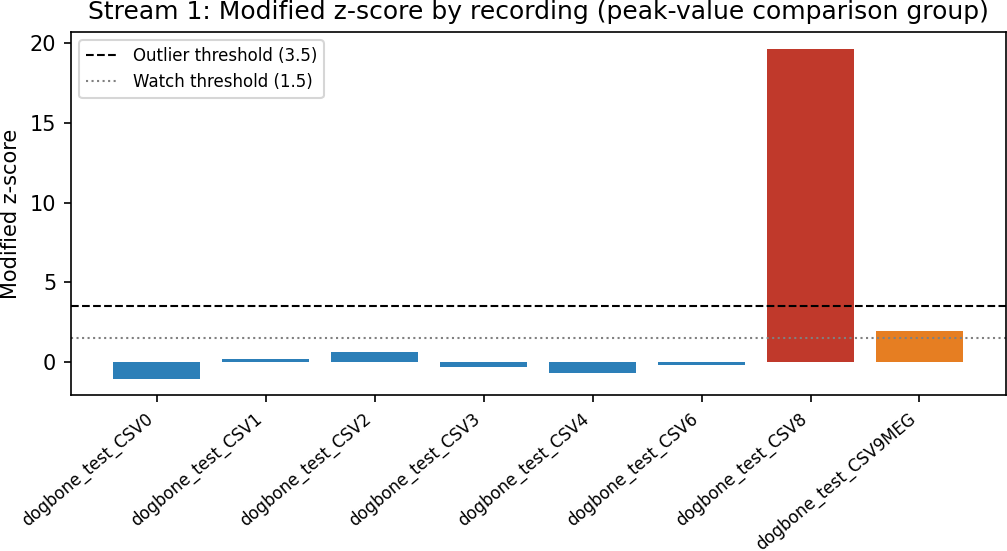
\includegraphics[width=0.85\textwidth]{figs/fig_stream1_zscore.png}
\caption{Modified $z$-score per AE summary recording (Section~3.3.2), computed directly from the raw sensor exports. Red and orange bars mark Proxy-Yes and Watch classifications; dashed lines mark the 1.5 and 3.5 thresholds.}
\label{fig:zscore}
\end{figure}

In summary, three of the ten AE recordings (30\%) show a proxy fracture signature at medium confidence or above, one of them (10\%) at high confidence based on genuine multi-sensor burst-timing evidence, and seven show no meaningful deviation from baseline acoustic activity. This distribution is broadly consistent with what one would expect if genuine fracture events are relatively rare within any given batch of tensile tests, rather than either universal or vanishingly unlikely, which lends some indirect plausibility to the proxy method's output, even though it cannot be checked against a confirmed label.

\subsection{Stream 2 --- Literature Dataset Results}
The final dataset comprises 129 samples across ten papers. Of these, 114 (88.4\%) report ``Yes'' cracking and 15 (11.6\%) report ``No'': IN939 was reported crack-free in fewer than one in eight published conditions. This imbalance is consistent across essentially all ten sources individually, reinforcing the characterisation of Section~2.1 of IN939 as an alloy that cracks under most attempted LPBF conditions, largely independently of laboratory, platform or parameter range; it is this consistency across independent sources, rather than the aggregate figure alone, that gives the 88.4\% base rate its credibility. Broken down by source (Table~\ref{tab:sources}), six of the ten papers report a 100\% cracking rate among their own samples, and the other four report mixed outcomes. The lowest crack proportions (33\%) occur in the two sources with the highest share of doped samples, reinforcing at the level of raw counts, rather than any model, the doping-status pattern that the SHAP analysis later identifies as the dominant predictive feature.

\subsection{Stream 3 --- Model Performance and Explainability}
\subsubsection{Cross-Validated Performance}
Across five-fold stratified cross-validation, the model achieved 92.2\% accuracy (119 of 129 correctly classified). Table~\ref{tab:confusion} gives the confusion matrix and Figure~\ref{fig:confusion} its heatmap.

\begin{table}[t]
\centering
\small
\begin{adjustbox}{max width=\textwidth,center}
\begin{tabular}{llcc}
\toprule
 & & Predicted: No & Predicted: Yes \\
\midrule
Actual: No (n=15) & & 11 (correct) & 4 (missed) \\
Actual: Yes (n=114) & & 6 (missed) & 108 (correct) \\
\bottomrule
\end{tabular}
\end{adjustbox}
\caption{Confusion matrix, aggregated across the five held-out cross-validation folds (129 samples total).}
\label{tab:confusion}
\end{table}

\begin{figure}[t]
\centering
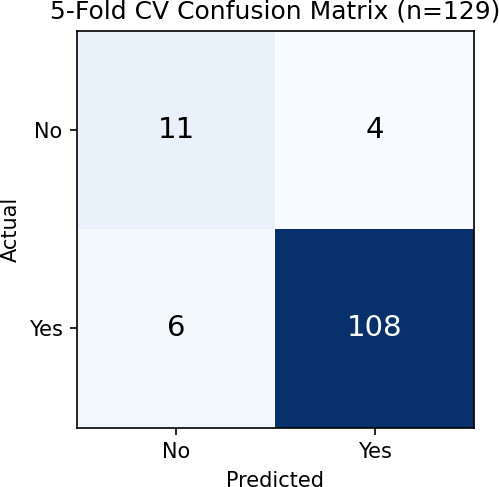
\includegraphics[width=0.38\textwidth]{figs/fig_confusion.png}
\caption{Confusion matrix heatmap for the same five-fold cross-validated predictions reported in Table~\ref{tab:confusion}.}
\label{fig:confusion}
\end{figure}

On the minority ``No-crack'' class, the harder and more practically important class given the safety implications, precision was 0.65 and recall 0.73: of fifteen genuine no-crack samples, eleven were correctly identified and four missed. This is reported as the direct, honest cost of class imbalance rather than minimised: with only fifteen true no-crack examples across the entire literature gathered, a handful of misclassifications represents a substantial share of the available minority-class evidence, and the headline 92.2\% accuracy figure alone would obscure this if reported without the class-level breakdown. For comparison, a naive classifier that simply predicted ``cracked'' for every sample would achieve 88.4\% accuracy, close to the trained model's 92.2\% headline figure, which underscores why accuracy alone is a misleading metric for an imbalanced dataset of this kind, and why the class-level precision and recall figures are reported here as the more informative measure of the model's genuine discriminative ability.

Concretely, each of the 129 samples was predicted by a model version trained on the other four folds, meaning it had never seen that sample during training. Of the fifteen true no-crack samples (spread roughly three per fold), eleven received a correct prediction and four an incorrect ``Yes''; of the 114 true crack samples, 108 were correct and six were missed. These ten misclassifications underlie the 92.2\% headline figure, and Section~5.6 discusses why the four missed no-crack cases matter disproportionately, given how scarce genuine no-crack examples are in the wider literature. Inspecting which samples were misclassified shows no single obvious pattern: the four missed no-crack samples span three different papers and a range of VED values, suggesting the errors are not concentrated in one poorly represented region of the feature space but instead reflect the general difficulty of the minority class given how few examples of it there are to learn from.

\subsubsection{SHAP Feature Importance}
Table~\ref{tab:shap} reports the mean absolute SHAP value per feature, averaged across all 129 samples, and Figure~\ref{fig:shap} shows the beeswarm plot.

\begin{table}[t]
\centering
\small
\begin{adjustbox}{max width=\textwidth,center}
\begin{tabular}{lcl}
\toprule
Feature & Mean $|$SHAP$|$ & Relative influence \\
\midrule
Doping status & 0.194 & Strongest predictor, over 2$\times$ the next feature \\
Layer thickness & 0.091 & Second strongest \\
Laser power & 0.071 & --- \\
Hatch spacing & 0.068 & --- \\
Scan speed & 0.036 & --- \\
VED (composite) & 0.024 & Weakest of the six features \\
\bottomrule
\end{tabular}
\end{adjustbox}
\caption{SHAP feature importance (mean absolute SHAP value across all 129 training samples), ranked by influence on the model's crack-risk prediction.}
\label{tab:shap}
\end{table}

\begin{figure}[t]
\centering
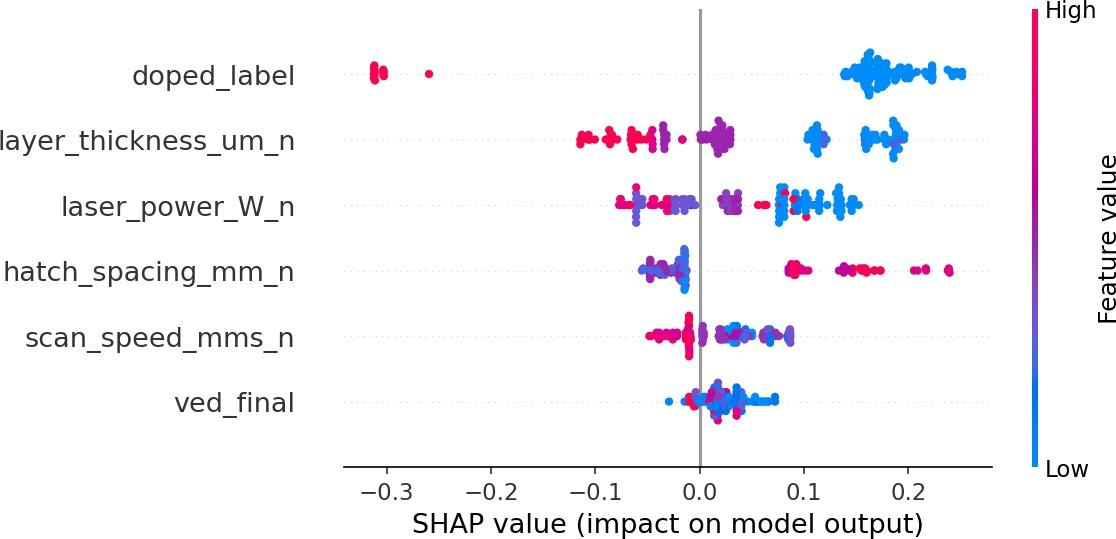
\includegraphics[width=0.85\textwidth]{figs/fig_shap.png}
\caption{SHAP summary (beeswarm) plot for the trained Random Forest classifier, generated directly from the fitted model and the 129-sample training set.}
\label{fig:shap}
\end{figure}

Doping status is, by a clear margin, the most influential feature: its mean absolute SHAP value (0.194) is more than double that of the next feature (layer thickness, 0.091) and more than eight times VED itself (0.024). Doped samples are consistently associated with lower predicted crack risk, directly consistent with Section~2.4. Among the four process parameters, layer thickness and laser power show the largest influence, hatch spacing similar, scan speed lower. VED, despite combining all four, ranks lowest of all six features, a somewhat counterintuitive result given how central VED is to the process-parameter literature reviewed in Section~2.3, but consistent with that literature's own finding that VED alone is an incomplete predictor of outcome. One plausible explanation is that VED, being a ratio of four other features already in the model, carries information the model can already pull from those four features directly. The Random Forest may therefore be spreading the predictive signal that a human reading a single VED number would attribute to VED across its four constituent parameters instead, a natural consequence of including both the composite metric and its components as separate features.

\subsubsection{Application to Real Specimens}
The trained model was applied to the two estimated conditions from \citet{marchese2020} (Table~\ref{tab:specimen}): lowest crack density (VED $\approx 88.0$\,J/mm$^3$) and lowest porosity (VED $\approx 158.3$\,J/mm$^3$), both non-doped, consistent with the real specimens available.

\begin{table}[t]
\centering
\small
\begin{adjustbox}{max width=\textwidth,center}
\begin{tabular}{lccc}
\toprule
Estimated condition (density-cube specimens) & VED (J/mm$^3$) & P(crack) & Prediction \\
\midrule
Lowest-cracking-density recipe \citep{marchese2020} & 88.0 & 1.00 & Yes \\
Lowest-porosity recipe \citep{marchese2020} & 158.3 & 1.00 & Yes \\
\bottomrule
\end{tabular}
\end{adjustbox}
\caption{Model predictions applied to the real density-cube specimens, using two estimated reference recipes (both non-doped).}
\label{tab:specimen}
\end{table}

Both conditions were predicted at 1.00 crack probability. This lines up with the dataset's 88.4\% base rate: given a non-doped composition, the factor SHAP identifies as most strongly associated with crack outcomes, a high prediction is expected regardless of VED, which limits how much this specific prediction can discriminate between the two conditions. Section~5.3 returns to this critically. It is worth noting that this ceiling effect is itself an interpretable, and in a sense reassuring, model behaviour: rather than producing an arbitrary or unstable prediction when pushed outside the exact conditions it was trained on, the model falls back sensibly on the dominant feature it has learned to trust most. That is consistent behaviour, not a failure mode, even though it limits how discriminative this particular prediction is.

\subsection{Comparing the Two Independent Crack-Risk Estimates}
It is important to state precisely what can and cannot be concluded from placing the Stream~1 and Stream~3 results side by side. These are not two measurements of the same physical specimen: Stream~1's AE evidence comes from tensile dogbone specimens, while Stream~3 was applied to conditions for the separate density-cube specimens. They cannot be combined into a single confirmed finding about one physical part, and are not presented as such. What can honestly be said is that both independent lines of evidence, one grounded in real measured signals, the other in a model trained across the literature, point in the same qualitative direction: elevated crack risk, consistent with IN939's generally crack-prone character. This is a reassuring consistency check, not a validated joint result, and the distinction between the two is maintained deliberately throughout the reporting. A reader tempted to treat this agreement as stronger evidence than it is should note that both estimates share a common bias in the same direction: IN939 is reported as crack-prone across the great majority of the literature, and the real specimens are non-doped, so both Stream~1 and Stream~3 would be expected to lean towards ``elevated risk'' a priori even before any recording-specific or specimen-specific evidence is considered, which tempers how much independent weight their agreement should be given.

\subsection{Summary of Findings}
It has been established, with reasonable confidence given the dataset size and cross-validation, that a Random Forest trained on published IN939 literature predicts crack outcomes with 92.2\% accuracy, and that doping status is a substantially stronger predictor than any single process parameter or VED. It has also been established, independently of any model, that IN939 cracks in the substantial majority of published conditions, and that sources including doped samples tend to report lower crack proportions. It has not been established that any specific real specimen has been confirmed cracked or not: Stream~1 remains proxy inference, and the Stream~3 real-specimen application rests on estimated rather than measured parameters.

\section{Discussion}
\subsection{Interpretation of Findings in Relation to the Research Questions}
RQ1 asked what can be inferred about fracture events directly from raw signals without a confirmed label. Stream~1 shows a defensible answer is possible: the dual-channel burst-and-collapse signature is genuinely distinctive, not an arbitrary artefact, but confidence varies considerably with data resolution, from high where raw hit data exists to weaker where only a summary trace is available. RQ2 asked whether an explainable model can accurately predict crack outcomes from parameters; Stream~3 answers affirmatively, achieving 92.2\% cross-validated accuracy while surfacing a literature-consistent finding that doping outweighs VED and the individual parameters combined. RQ3 asked how proxy, literature-derived and measured evidence should be combined when ground truth is unavailable; the answer demonstrated throughout is to keep each source explicitly labelled by evidentiary status rather than blending them into one unqualified claim, even where they happen to agree (Section~4.5).

A further point reinforces the SHAP finding independently: Table~\ref{tab:sources} shows that every sample from the three non-doped, process-parameter-only studies reports cracking (27/27, 48/48, 3/3), while three of the four doped-sample studies report a materially lower crack proportion, visible directly in the raw literature data without any model. The model's SHAP conclusion and this simple source-level tabulation corroborate one another via two independent routes, strengthening confidence considerably beyond either alone. This triangulation, possible because per-source traceability was retained throughout the mining pipeline rather than only working with the pooled dataset, exemplifies the methodological-honesty principle: a striking model output is more trustworthy once shown to hold under a second, simpler, independent check that does not depend on the model at all.

\subsection{The Doping-Status Finding in Context}
That doping status dominates VED as a crack-risk predictor has a direct practical implication: for an organisation seeking to reduce IN939 cracking, compositional modification may offer a larger, more robust risk reduction than further VED optimisation alone, consistent with \citet{bae2025}, whose TiB$_2$ addition eliminated cracking entirely, compared with the narrower process windows of Section~2.3. The contribution here is not discovering this pattern for the first time, since each doping paper already reports a beneficial effect individually, but quantifying, via a model trained jointly across the literature, how much more influential this factor is relative to every other variable simultaneously: a cross-study comparison difficult to obtain from any single experimental paper working within its own narrower parameter set. For an organisation weighing where to invest limited development resources, this reframes the decision: rather than continuing to fund incremental parameter-optimisation studies within a single-digit-percentage-point improvement ceiling, the evidence assembled here suggests a compositional trial, even a modest one, is likely to yield a larger, more robust reduction in crack risk per unit of research effort invested. This inference is subject to the source-level confounding noted among the limitations below: all 13 doped samples come from four papers.

\subsection{Practical Implications and the Limits of the Real-Specimen Application}
Applying the trained model to real density-cube specimens illustrates both the promise and the limits of this approach. Obtaining a quantified, explainable crack-risk estimate without destructive testing or CT scanning is precisely the low-cost complement this work set out to explore. However, the result obtained, both conditions at 1.00 crack probability, is driven by their shared non-doped composition rather than differing VED values, meaning this application does not yet discriminate meaningfully between process windows for these specimens; it correctly places them in the alloy's high-risk region without the parameter-level nuance the model has demonstrably learned elsewhere. This is a direct consequence of the estimated-parameters limitation (Section~3.9), underlining that the most valuable near-term extension (Section~6) is obtaining the real, measured process parameters for these specimens, which would allow the model's finer-grained parameter sensitivity to be exercised properly rather than saturated by the dominant doping feature.

\subsection{Relating Stream 1 to the Wider In-Situ Monitoring Literature}
Section~2.5 established AE-based detection as physically well motivated, but existing applications, including the reinforcement-learning system of \citet{wasmer2019}, are trained against known labels, which are not available here. Stream~1's contribution sits specifically in this gap: rather than training against labelled examples, it applies the underlying physical principle (a genuine fracture produces a large, often multi-channel burst followed by a collapse) directly and manually, without any training step, where no labelled examples exist. This is deliberately more modest than a trained classifier: it cannot improve with more data, and its reliability rests entirely on how well established the underlying signature is, rather than on data-driven validation. The research gap identified in Section~2.7 is therefore addressed conservatively, falling back on first-principles signal physics rather than inventing labels or forcing an unsuitable trained-classifier approach onto data too scarce to support one.

This clarifies a deliberate division of labour: Stream~1 answers ``does this recording look like it captured a fracture'', using only that recording's own physics, while Stream~3 answers ``how likely is a fracture given this general set of conditions'', using the accumulated literature evidence. \citet{grasso2017} frame this as the distinction between signal-based (bottom-up) and model-based (top-down) defect-detection strategies; this work runs both in parallel deliberately, since each compensates for the other's limitation: Stream~1 provides direct physical grounding but cannot generalise beyond its ten recordings, while Stream~3 generalises across a much larger evidence base but is once removed from this project's own hardware and specimens. Neither stream alone would offer as complete a picture: Stream~1 without Stream~3 would leave the real recordings uninterpreted against any broader context of what ``typical'' IN939 crack rates look like, while Stream~3 without Stream~1 would leave this project's own laboratory data entirely unanalysed on its own terms.

\subsection{Cost and Practicality Considerations}
Given the motivating premise that in-situ and literature-based methods might complement existing inspection, the cost and time asymmetry is worth making explicit. CT scanning can take hours per part plus analysis time and requires specialist equipment; destructive sectioning permanently consumes the part. By contrast, the Stream~3 model can be queried in a fraction of a second at zero marginal cost, and Stream~1's analysis runs against data a production printer could already be recording, with no additional destructive step. Neither approach is yet accurate or validated enough to replace CT scanning or destructive testing outright; that requires the ground-truth validation recommended in Section~6. But even a partially reliable, appropriately caveated estimate has genuine value as a triage step, flagging which builds most warrant full CT inspection rather than replacing that inspection altogether, particularly in a development phase where many trial builds are produced in quick succession, when the cumulative cost of CT-scanning every single trial build would otherwise be prohibitive relative to the development budget typically available for parameter-optimisation work.

\subsection{Limitations Revisited}
The absence of confirmed ground truth means neither Stream~1's classifications nor Stream~3's real-specimen predictions can be presented as validated findings: both are well-reasoned, transparent estimates rather than confirmed detections. The small sensor sample size means Stream~1's results describe these ten specific recordings only, not a generalisable detection rate. The literature dataset's class imbalance means the model's no-crack performance (0.65 precision, 0.73 recall) is measurably weaker than the 92.2\% headline figure suggests, and any future application to novel conditions should weight this limitation heavily rather than quoting the headline accuracy alone. The estimated real-specimen parameters mean the Section~4.4.3 prediction should not be treated as equivalent to a prediction from this project's own confirmed print settings. Every limitation here is a deliberate feature of the methodological honesty of Section~3.6, not a flaw discovered after the fact.

Two further limitations concern the validation design. First, stratified five-fold cross-validation splits by sample and not by source paper, whereas samples from the same publication share a printer, powder batch and reporting conventions; this may overstate generalisation to an unseen publication. Second, all 13 doped samples come from only four papers, so doping status is partly confounded with source, and the SHAP ranking may partly reflect source-level differences. Cross-validation grouped by paper is a necessary next step. Finally, the LLM extraction was checked by consistency rules, evidence quotations and spot checks, but not by independent manual transcription of every field.

\subsection{Reflection on the Three-Stream Design as a Response to Data Scarcity}
The underlying situation this design addresses, real, physically grounded but unlabelled and too-scarce-to-model data alongside a larger but once-removed body of external labelled evidence, is common across applied engineering machine learning generally. Sensors are cheap to install and leave running, so raw data accumulates quickly, while confirmed outcome labels require a slower, more expensive verification step and lag behind. The response here (using scarce real data for direct physics-grounded reasoning where suited, using the larger external evidence base for training that scarce data cannot support, and explicitly reporting both rather than blending them) is offered as a reasonably general template applicable well beyond IN939 or even beyond metal additive manufacturing. Its central discipline, applicable beyond this project, is refusing to let the more statistically rigorous analysis silently absorb or overstate the authority of the more physically direct but less validated one, or vice versa.

\section{Conclusion and Future Work}
\subsection{Summary of Contributions}
This work investigated whether real-time sensor monitoring, published literature evidence and explainable machine learning could together provide a defensible, low-cost estimate of crack risk in IN939 LPBF components, given the consequential absence of confirmed ground-truth labels. Stream~1 developed and applied a physics-based proxy classification method to ten real AE recordings, identifying one high-confidence and two medium-confidence likely fracture events against seven showing no such signature. Stream~2 built a 129-sample structured literature dataset from ten sources via an LLM-assisted pipeline, confirming that the alloy cracks in 88.4\% of published conditions. Stream~3 trained and cross-validated a Random Forest achieving 92.2\% accuracy, establishing via SHAP that doping status is a considerably stronger crack-risk predictor than VED or any individual parameter, before applying the model to real specimens as a second, independent estimate.

Beyond these technical contributions, the broader contribution is an explicit approach to reporting evidence honestly when ground truth is unavailable: distinguishing statistically validated findings, well-reasoned but unconfirmed proxy inferences, and illustrative estimates resting on assumed rather than measured inputs. This distinction, and the two methodological decisions underpinning it (Section~3.6), were reviewed and approved by the supervisor, and are offered as a template for similarly data-constrained applied AI projects, particularly in engineering domains where sensor data is abundant but confirmed outcome labels remain scarce and expensive to obtain. The work therefore closes not with a single validated crack-detection tool, but with a working demonstration that literature-derived, explainable machine learning and physics-informed signal reasoning can be combined honestly and usefully even under exactly the conditions (scarce, unlabelled real data alongside a larger but once-removed literature base) that make this kind of applied AI problem genuinely difficult in practice, and with a clear, concrete set of next steps for closing the remaining gap to validated deployment.

\subsection{Recommendations for Future Work}
Three extensions follow directly from Section~5.6. First, obtaining confirmed post-build inspection (CT scanning or sectioning) for the real specimens analysed here would allow both Stream~1 and Stream~3 estimates to be validated against genuine ground truth for the first time, closing the single largest gap identified throughout. Second, recording actual process parameters for future real specimens at print time, rather than estimating retrospectively as Section~3.5.3 required, would remove the largest source of uncertainty in the real-specimen application. Third, synchronising acoustic and thermal (and potentially optical) recordings from the same physical specimens with a shared timestamp reference would finally enable the genuine multi-modal sensor fusion that this project's original title anticipated.

Beyond these, a longer-term direction would be to keep growing the literature dataset as new IN939 studies come out, particularly further doping studies given their outsized influence, and revisit the model's performance as that evidence base grows, including evaluation with cross-validation grouped by source paper. A sufficiently matured, ground-truth-validated version of this pipeline would represent a publishable contribution to explainable, sensor-informed defect prediction for difficult-to-print superalloys.

For the laboratory specifically, three low-cost changes to data-collection practice would remove the largest uncertainties identified here without new equipment. First, logging a simple pass/fail note at inspection time would close the ground-truth gap that has been this work's central limitation, at negligible cost. Second, recording exact process parameters alongside each specimen identifier would remove the need for the estimated-parameter substitution used here. Third, adopting a shared timestamp reference whenever both acoustic and thermal sensors monitor the same build would directly enable the multi-modal fusion this work's title anticipated for future specimens, at minimal additional overhead to existing data-collection practice.

\section*{Declarations}
\paragraph{Data and code availability.} All code to reproduce the literature-mining pipeline, sensor-data processing and modelling and SHAP analysis, along with an interactive results dashboard, is available in the project repository (IN939-LPBF-Crack-Detection). The source papers used for LLM-assisted literature extraction are not included in the repository for copyright reasons and would need to be downloaded separately. Raw acoustic-emission and thermal sensor recordings are not included because they have not been cleared for public release. The cleaned literature-mined dataset used to train and back-test the models is supplied in the repository as \texttt{clean\_dataset\_125.csv}.

\paragraph{Ethics.} The study used publicly available secondary data and laboratory-internal engineering data with no personal information and involved no human participants. Ethical approval was waived by the project supervisor under the university's supervisor delegated approval process.

\paragraph{Acknowledgements.} The author thanks the project supervisor, Professor Gregory Gibbons, for guidance and for reviewing the methodological decisions described in this paper, and the laboratory contact who supplied the sensor recordings.

\begin{thebibliography}{99}
\setlength{\itemsep}{4pt}\small
\bibitem[Bae et al.(2025)]{bae2025}
Bae, J.-S., Tekoglu, E., Alrizqi, M., O'Brien, A.D., Liu, J., Biggs, K., Kim, S.Y., Penn, A., Šulák, I., Chen, W., So, K.P., Hart, A.J., Sim, G.-D. and Li, J. (2025) ``Additive manufacturing of strong and ductile In939+TiB2 by laser powder bed fusion,'' Materials Science and Engineering: A, 939, 148446. DOI: 10.1016/j.msea.2025.148446.

\bibitem[Breiman(2001)]{breiman2001}
Breiman, L. (2001) ``Random Forests,'' Machine Learning, 45(1), pp. 5--32. DOI: 10.1023/A:1010933404324.

\bibitem[Chen et al.(2026)]{chen2026}
Chen, C., Lu, L. and Wang, T. (2026) ``Effect of TiC particles on the microstructure and properties of Inconel 939 processed by selective laser melting,'' Journal of Materials Research, 41(9), pp. 1373--1390. DOI: 10.1557/s43578-026-01841-6.

\bibitem[Ding et al.(2026)]{ding2026}
Ding, H., Zhang, X., Emanet, S., Chen, Y., Bagheri, E., Mu, Y., Meng, W.J. and Guo, S. (2026) ``Dual-doped IN939 superalloy with superior strength and high temperature oxidation resistance via Laser Powder Bed Fusion,'' Materials Science and Engineering: A, 961, 150144. DOI: 10.1016/j.msea.2026.150144.

\bibitem[Doğu et al.(2024)]{dogu2024}
Doğu, M.N., Obeidi, M.A., Gu, H., Teng, C. and Brabazon, D. (2024) ``Powder Bed Fusion--Laser Beam of IN939: The Effect of Process Parameters on the Relative Density, Defect Formation, Surface Roughness and Microstructure,'' Materials, 17(13), 3324. DOI: 10.3390/ma17133324.

\bibitem[Grasso and Colosimo(2017)]{grasso2017}
Grasso, M. and Colosimo, B.M. (2017) ``Process defects and in situ monitoring methods in metal powder bed fusion: a review,'' Measurement Science and Technology, 28(4), 044005. DOI: 10.1088/1361-6501/aa5c4f.

\bibitem[Hu et al.(2024)]{hu2024}
Hu, P., Liu, Z., Zhang, H., Li, Y., Zhou, Q. and Xie, J. (2024) ``Effect of remelting on cracking of Inconel 939 fabricated via laser powder bed fusion,'' Materials Characterization, 214, 114087. DOI: 10.1016/j.matchar.2024.114087.

\bibitem[Iglewicz and Hoaglin(1993)]{iglewicz1993}
Iglewicz, B. and Hoaglin, D.C. (1993) How to Detect and Handle Outliers, ASQC Basic References in Quality Control: Statistical Techniques, Vol. 16. Milwaukee, WI: ASQC Quality Press.

\bibitem[Li et al.(2024/2025)]{li2024}
Li, S., Gao, S., Zhang, W., Lu, G., Cui, L., Li, L., Ma, Y. and Wang, S. (2024) ``Study of the Crack and Porosity Regulation of a Non-weldable Ni-Based Superalloy Fabricated by Laser Powder Bed Fusion,'' Journal of Materials Engineering and Performance, 34(15), pp. 15854--15865. DOI: 10.1007/s11665-024-10362-4.

\bibitem[Lundberg and Lee(2017)]{lundberg2017}
Lundberg, S.M. and Lee, S.-I. (2017) ``A Unified Approach to Interpreting Model Predictions,'' Advances in Neural Information Processing Systems 30 (NeurIPS 2017), pp. 4765--4774.

\bibitem[Marchese et al.(2020)]{marchese2020}
Marchese, G., Parizia, S., Saboori, A., Manfredi, D., Lombardi, M., Fino, P., Ugues, D. and Biamino, S. (2020) ``The Influence of the Process Parameters on the Densification and Microstructure Development of Laser Powder Bed Fused Inconel 939,'' Metals, 10(7), 882. DOI: 10.3390/met10070882.

\bibitem[Ozer et al.(2024)]{ozer2024}
Ozer, S., Doğu, M.N., Ozdemirel, C., Bilgin, G.M., Gunes, M., Davut, K., Gu, H. and Brabazon, D. (2024) ``Effect of aging treatment on the microstructure, cracking type and crystallographic texture of IN939 fabricated by powder bed fusion-laser beam,'' Journal of Materials Research and Technology, 33, pp. 574--588. DOI: 10.1016/j.jmrt.2024.09.106.

\bibitem[Rodríguez-Barber et al.(2023)]{rodriguezbarber2023}
Rodríguez-Barber, I., Fernández-Blanco, A.M., Unanue-Arruti, I., Madariaga-Rodríguez, I., Milenkovic, S. and Pérez-Prado, M.T. (2023) ``Laser powder bed fusion of the Ni superalloy Inconel 939 using pulsed wave emission,'' Materials Science and Engineering: A, 870, 144864. DOI: 10.1016/j.msea.2023.144864.

\bibitem[Wasmer et al.(2019)]{wasmer2019}
Wasmer, K., Le-Quang, T., Meylan, B. and Shevchik, S.A. (2019) ``In Situ Quality Monitoring in AM Using Acoustic Emission: A Reinforcement Learning Approach,'' Journal of Materials Engineering and Performance, 28(2), pp. 666--672. DOI: 10.1007/s11665-018-3690-2.

\bibitem[Zhang et al.(2023)]{zhang2023}
Zhang, B., Ding, H., Meng, A.C., Nemati, S., Guo, S. and Meng, W.J. (2023) ``Crack reduction in Inconel 939 with Si addition processed by laser powder bed fusion additive manufacturing,'' Additive Manufacturing, 72, 103623. DOI: 10.1016/j.addma.2023.103623.

\end{thebibliography}

\end{document}
